\documentclass[12pt,a4paper]{article}

\usepackage{fontspec}
\defaultfontfeatures{Ligatures=TeX}
\usepackage{polyglossia}
\setdefaultlanguage{russian}
\setotherlanguage{english}
\setmainfont{Times New Roman}
\setsansfont{Arial}
\setmonofont{Courier New}
\newfontfamily\cyrillicfont{Times New Roman}
\newfontfamily\cyrillicfontsf{Arial}
\newfontfamily\cyrillicfonttt{Courier New}
\usepackage{amsmath,amssymb}
\usepackage{mathtools}
\usepackage{booktabs}
\usepackage{graphicx}
\usepackage{hyperref}
\usepackage{xcolor}
\usepackage[margin=2.5cm]{geometry}

\hypersetup{
  colorlinks=true,
  linkcolor=blue!60!black,
  citecolor=blue!60!black,
  urlcolor=blue!60!black,
  pdfauthor={Давид Алфёров},
  pdftitle={Нелокальные однопетлевые формфакторы спектрального действия с содержанием частиц Стандартной модели},
  pdfsubject={doi:10.22541/au.177507193.33027854/v1}
}

%%% Custom commands
\newcommand{\Weylsq}{C_{\mu\nu\rho\sigma}C^{\mu\nu\rho\sigma}}
\newcommand{\Ricsq}{R_{\mu\nu}R^{\mu\nu}}
\newcommand{\Riemsq}{R_{\mu\nu\rho\sigma}R^{\mu\nu\rho\sigma}}
\newcommand{\dd}{\mathrm{d}}
\newcommand{\erfi}{\operatorname{erfi}}
\newcommand{\tr}{\operatorname{tr}}
\newcommand{\Tr}{\operatorname{Tr}}

\begin{document}

\title{Нелокальные однопетлевые формфакторы спектрального действия\\с содержанием частиц Стандартной модели}

\author{Давид Алфёров\footnote{E-mail: davidich.alfyorov@gmail.com}}

\date{}

\maketitle

\begin{abstract}
Мы вычисляем полные нелокальные однопетлевые формфакторы $F_1(\Box/\Lambda^2)$
и $F_2(\Box/\Lambda^2,\xi)$ квадратичного по кривизне сектора спектрального
действия $S = \Tr\,f(D^2/\Lambda^2)$ для всего содержания частиц Стандартной
модели: 4 вещественных скаляра (дублет Хиггса), $45/2$ дираковских
фермионов (3 поколения) и 12 калибровочных бозонов
($\mathrm{SU}(3)\times\mathrm{SU}(2)\times\mathrm{U}(1)$).
С~помощью ковариантной теории возмущений Барвинского--Вилковыского и
диаграммного ядра теплопроводности Коделло--Занусси мы получаем
результаты в замкнутой форме для каждого спинового сектора (0, 1/2, 1)
в вейлевском базисе $\{C^2, R^2\}$ и собираем полные суммы Стандартной модели.
Локальные пределы, определяемые стандартными коэффициентами
ядра теплопроводности~\cite{Gilkey:1975iq,Vassilevich:2003xt}, дают
$\alpha_C = 13/120$ для коэффициента при квадрате тензора Вейля и
$\alpha_R(\xi) = 2(\xi-1/6)^2$ для коэффициента при $R^2$, где $\xi$ ---
параметр неминимальной связи поля Хиггса. Показано, что оба формфактора
являются целыми функциями переменной $\Box/\Lambda^2$, что гарантирует
отсутствие дополнительных полюсов пропагатора помимо имеющихся в
классической теории.
Мы выводим отношение $c_1/c_2$ в базисе $\{R^2, R_{\mu\nu}^2\}$, условие
отщепления скалярного гравитона при конформной связи $\xi = 1/6$, а также
ультрафиолетовое асимптотическое поведение. Формфакторы приводят к
модифицированному ньютоновскому потенциалу с вычисляемыми
эффективными массами $m_2 = \Lambda\sqrt{60/13}$ и
$m_0 = \Lambda/\sqrt{6(\xi-1/6)^2}$, связывая формализм спектрального
действия с феноменологией Солнечной системы. Все результаты подтверждены
независимыми численными вычислениями с произвольной арифметической точностью.
\end{abstract}

\textit{Ключевые слова:} спектральное действие, ядро теплопроводности, формфакторы,
квадратичная гравитация, Стандартная модель, некоммутативная геометрия.

\bigskip
\selectlanguage{english}
\textbf{Nonlocal one-loop form factors of the spectral action with Standard Model content}

\textbf{Abstract.}
We compute the complete nonlocal one-loop form factors $F_1(\Box/\Lambda^2)$
and $F_2(\Box/\Lambda^2,\xi)$ of the curvature-squared sector of the spectral
action $S = \Tr\,f(D^2/\Lambda^2)$ for the full Standard Model particle content:
4 real scalars (Higgs), $45/2$ Dirac-equivalent fermions (3 generations), and
12 gauge bosons ($\mathrm{SU}(3)\times\mathrm{SU}(2)\times\mathrm{U}(1)$).
Using the Barvinsky--Vilkovisky covariant perturbation theory and the
Codello--Zanusso diagrammatic heat kernel, we derive closed-form results for
each spin sector (0, 1/2, 1) in the $\{C^2, R^2\}$ Weyl basis and assemble the
Standard Model totals. The local limits, determined by standard heat kernel
coefficients~\cite{Gilkey:1975iq,Vassilevich:2003xt}, yield
$\alpha_C = 13/120$ for the Weyl-squared coefficient and
$\alpha_R(\xi) = 2(\xi-1/6)^2$ for the $R^2$ coefficient, where $\xi$ is the
Higgs non-minimal coupling. Both form factors are shown to be entire functions
of $\Box/\Lambda^2$, ensuring that the one-loop effective action introduces no
additional propagator poles beyond those of the classical theory.
We derive the $c_1/c_2$ ratio in the $\{R^2, R_{\mu\nu}^2\}$ basis, the scalar
graviton decoupling condition at conformal coupling $\xi = 1/6$, and the UV
asymptotic behavior. The form factors yield a modified Newtonian potential with
calculable effective masses $m_2 = \Lambda\sqrt{60/13}$ and
$m_0 = \Lambda/\sqrt{6(\xi-1/6)^2}$, connecting the spectral action framework
to solar-system phenomenology. All results are verified by independent
multi-precision numerical evaluation.

\textit{Keywords:} spectral action, heat kernel, form factors, quadratic gravity,
Standard Model, noncommutative geometry.
\selectlanguage{russian}


% ============================================================
\section{Введение}
\label{sec:intro}
% ============================================================

Принцип спектрального действия~\cite{Chamseddine:1996zu,Chamseddine:2006ep}
обеспечивает геометрическое происхождение как гравитационных, так и
калибровочных взаимодействий: бозонное действие задаётся выражением
$S = \Tr\,f(D^2/\Lambda^2)$, где $D$ --- оператор Дирака некоммутативной
геометрии, $\Lambda$ --- спектральный масштаб обрезания, а $f$ --- положительная
чётная функция. На классическом уровне разложение этого следа по ядру
теплопроводности воспроизводит действие Эйнштейна--Гильберта, космологическую
постоянную и члены Янга--Миллса из первых нескольких коэффициентов
Сили--ДеВитта~\cite{Chamseddine:2010ud,vanSuijlekom:2014pya}.

За рамками ведущего приближения Сили--ДеВитта спектральное действие порождает
\emph{нелокальные} квадратичные по кривизне члены, характеризуемые зависящими
от импульса формфакторами $F_1(\Box/\Lambda^2)$ и $F_2(\Box/\Lambda^2)$. Эти
формфакторы описывают полное однопетлевое квантово-гравитационное эффективное
действие порядка $\mathcal{O}(\mathcal{R}^2)$ и определяют модифицированный
пропагатор гравитона, спектр массивных гравитационных мод и ультрафиолетовое
поведение теории.

Ковариантная теория возмущений Барвинского--Вилковыского
(БВ)~\cite{Barvinsky:1985an,Barvinsky:1987uw} предоставляет общий формализм
для вычисления таких формфакторов для произвольного обобщённого лапласиана
$\Delta = -(g^{\mu\nu}\nabla_\mu\nabla_\nu + E)$ на векторном расслоении над
искривлённым многообразием. Диаграммная техника ядра теплопроводности
Коделло--Занусси (КЗ)~\cite{Codello:2012kq} даёт явные выражения для пяти
независимых формфакторов ($f_{\text{Ric}}, f_R, f_{RU}, f_U, f_\Omega$)
через универсальную мастер-функцию $\varphi(x)$. Коэффициенты Сили--ДеВитта
и их роль в спектральной геометрии обсуждаются
в~\cite{DeWitt:1964mxt,Gilkey:1975iq,Vassilevich:2003xt,Avramidi:2000bm,Fursaev:2011zz}.

В~предшествующих работах формфакторы вычислялись для отдельных спиновых
секторов~\cite{Barvinsky:1987uw,Codello:2012kq} или для упрощённого набора
частиц~\cite{Codello:2008vh}. В~настоящей статье мы представляем первое полное
вычисление для всего спектра Стандартной модели (СМ): 4 вещественных скаляра
(дублет Хиггса), $N_f = 45$ вейлевских фермионов (что эквивалентно
$N_D = 45/2$ дираковским фермионам) и 12 калибровочных бозонов группы
$\mathrm{SU}(3) \times \mathrm{SU}(2) \times \mathrm{U}(1)$. Соглашение
о~подсчёте следует работе Коделло, Перкаччи и Рахмеде
(КПР)~\cite{Codello:2008vh}.

Основные результаты:
\begin{itemize}
\item Замкнутые выражения для $h_C^{(s)}(x)$ и $h_R^{(s)}(x)$ при
  $s = 0, 1/2, 1$ в вейлевском базисе $\{C^2, R^2\}$ с корректным вычитанием
  духов для спина~1.
\item Полные суммы СМ: $\alpha_C = 13/120$ (фиксировано содержанием СМ) и
  $\alpha_R(\xi) = 2(\xi - 1/6)^2$ (зависит только от параметра неминимальной
  связи Хиггса~$\xi$).
\item Доказательство того, что $F_1$ и $F_2$ являются целыми функциями
  переменной $z = \Box/\Lambda^2$, что гарантирует отсутствие новых полюсов
  помимо унаследованных от структуры пропагатора.
\item Отношение $c_1/c_2$, отщепление скалярного гравитона при $\xi = 1/6$
  и ультрафиолетовая асимптотика.
\end{itemize}

Структура статьи следующая. В~разделе~\ref{sec:setup} устанавливаются
соглашения и излагается формализм БВ/КЗ. В~разделах~\ref{sec:scalar}--\ref{sec:vector} выводятся формфакторы для каждого спинового сектора.
В~разделе~\ref{sec:sm} собираются полные суммы СМ и выводятся их свойства.
В~разделе~\ref{sec:properties} обсуждается природа целых функций,
ультрафиолетовое поведение и эффективные массы гравитонов.
В~разделе~\ref{sec:discussion} проводится сравнение с~существующими результатами
и обсуждаются следствия. Заключение приведено в~разд.~\ref{sec:conclusions}.

В~данной статье мы используем евклидову сигнатуру $(+,+,+,+)$, естественные
единицы $c = \hbar = 1$ и соглашение для обобщённого лапласиана
$\Delta = -(g^{\mu\nu}\nabla_\mu\nabla_\nu + E)$ Барвинского и
Вилковыского~\cite{Barvinsky:1985an}. Лоренцево продолжение к сигнатуре
$(-,+,+,+)$ обсуждается в~разд.~\ref{sec:discussion}. Сводка основных
результатов приведена в~таблице~\ref{tab:summary}.


% ============================================================
\section{Постановка задачи и соглашения}
\label{sec:setup}
% ============================================================

\subsection{Обобщённый лапласиан и спектральное действие}

Рассмотрим замкнутое (компактное, без края) римановое спиновое
4-многообразие $(M,g)$. Спектральное действие в порядке
$\mathcal{O}(\mathcal{R}^2)$ в вейлевском базисе имеет вид
\begin{equation}
  S_{\text{spec}}\Big|_{\mathcal{R}^2}
  = \int_M \dd^4x\,\sqrt{g}\,\bigl[
    F_1(z)\,\Weylsq + F_2(z,\xi)\,R^2
  \bigr]\,,
  \label{eq:spectral-action}
\end{equation}
где $z \equiv \Box/\Lambda^2$ и $\Lambda$ --- спектральный масштаб обрезания.
Для обобщённого лапласиана $\Delta = -(g^{\mu\nu}\nabla_\mu\nabla_\nu + E)$,
действующего на векторном расслоении ранга $d_V$ (так что $\tr\,\mathbf{1} = d_V$),
эндоморфизм КЗ равен $\mathbf{U} = -E$, а кривизна расслоения ---
$\Omega_{\mu\nu} = [\nabla_\mu, \nabla_\nu]$.

\subsection{Мастер-функция}

Все формфакторы строятся из универсальной мастер-функции
\begin{equation}
  \varphi(x) = \int_0^1 \dd\xi\, e^{-\xi(1-\xi)x}\,,
  \label{eq:phi-def}
\end{equation}
имеющей замкнутую форму
\begin{equation}
  \varphi(x) = e^{-x/4}\sqrt{\frac{\pi}{x}}\;\erfi\!\left(\frac{\sqrt{x}}{2}\right)\,.
  \label{eq:phi-closed}
\end{equation}
Основные свойства:
$\varphi(0) = 1$,
$\varphi'(0) = -1/6$,
тейлоровские коэффициенты $a_n = (-1)^n\,n!/(2n+1)!$, так что
$\varphi(x) = \sum_{n=0}^\infty a_n\,x^n$ с бесконечным радиусом
сходимости. В~частности, $\varphi$ является целой функцией первого порядка
(рис.~\ref{fig:phi}).

\begin{figure}[t]
  \centering
  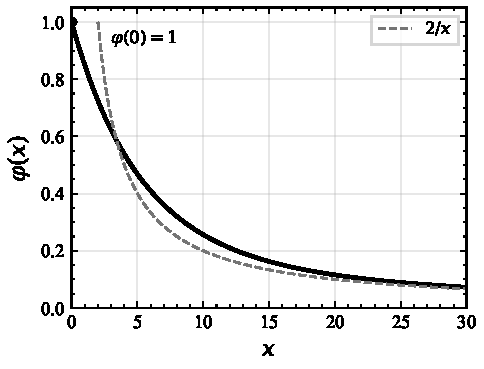
\includegraphics[width=0.8\textwidth]{figures/fig_phi_ru.pdf}
  \caption{Мастер-функция $\varphi(x)$, где
  $x = \Box/\Lambda^2$. Начиная с~$\varphi(0) = 1$, функция
  монотонно убывает и стремится к асимптотической форме $2/x$
  (штриховая линия) при $x \gg 1$.}
  \label{fig:phi}
\end{figure}

\subsection{Формфакторы КЗ}

Пять формфакторов КЗ~\cite{Codello:2012kq}:
\begin{subequations}
\label{eq:CZ-ff}
\begin{align}
  f_{\text{Ric}}(x) &= \frac{1}{6x} + \frac{\varphi - 1}{x^2}\,,
  \label{eq:fRic}\\
  f_R(x) &= \frac{\varphi}{32} + \frac{\varphi}{8x}
    - \frac{7}{48x} - \frac{\varphi - 1}{8x^2}\,,
  \label{eq:fR}\\
  f_{RU}(x) &= -\frac{\varphi}{4} - \frac{\varphi - 1}{2x}\,,
  \label{eq:fRU}\\
  f_U(x) &= \frac{\varphi}{2}\,,
  \label{eq:fU}\\
  f_\Omega(x) &= -\frac{\varphi - 1}{2x}\,.
  \label{eq:fOmega}
\end{align}
\end{subequations}
Их локальные пределы: $f_{\text{Ric}}(0) = 1/60$, $f_R(0) = 1/120$,
$f_{RU}(0) = -1/6$, $f_U(0) = 1/2$, $f_\Omega(0) = 1/12$.

\subsection{Сборка в вейлевском базисе}

Для любого спинового сектора формфакторы $\{C^2, R^2\}$ получаются из
формфакторов КЗ с~помощью правил сборки БВ. Детали зависят от
эндоморфизма $\mathbf{U}$, кривизны расслоения $\Omega_{\mu\nu}$ и
тождеств для следов, специфичных для каждого
спина~\cite{Barvinsky:1987uw,Parker:2009uva}.
Результат записывается в виде
\begin{equation}
  F_i^{(s)}(z) = \frac{h_i^{(s)}(z)}{16\pi^2}\,,\quad i = C, R\,,
  \label{eq:Fi-hi}
\end{equation}
где $s = 0, 1/2, 1$ обозначает спин, а $h_C^{(s)}, h_R^{(s)}$ --- приведённые
формфакторы. Локальные пределы $\beta_W^{(s)} \equiv h_C^{(s)}(0)$ и
$\beta_R^{(s)} \equiv h_R^{(s)}(0)$ представляют собой однопетлевые
коэффициенты $\beta$-функции операторов $C^2$ и $R^2$.


% ============================================================
\section{Спин 0: вещественный скаляр}
\label{sec:scalar}
% ============================================================

Для вещественного скалярного поля с~неминимальной связью $\xi R\phi^2/2$
обобщённый лапласиан имеет $\tr\,\mathbf{1} = 1$, $\mathbf{U} = \xi R$ и
$\Omega_{\mu\nu} = 0$ (тривиальное расслоение). Сборка БВ даёт
\begin{subequations}
\label{eq:scalar-ff}
\begin{align}
  h_C^{(0)}(x) &= \frac{1}{12x} + \frac{\varphi - 1}{2x^2}\,,
  \label{eq:hC0}\\
  h_R^{(0)}(x,\xi) &= f_{R,\text{bis}}(x)
    + \xi\,f_{RU}(x) + \xi^2\,f_U(x)\,,
  \label{eq:hR0}
\end{align}
\end{subequations}
где $f_{R,\text{bis}} = \tfrac{1}{3}f_{\text{Ric}} + f_R$.
Локальные пределы:
\begin{equation}
  \beta_W^{(0)} = \frac{1}{120}\,,\qquad
  \beta_R^{(0)}(\xi) = \frac{1}{2}\left(\xi - \frac{1}{6}\right)^{\!2}\,.
  \label{eq:beta-scalar}
\end{equation}
Формфакторы отдельных спиновых секторов показаны на
рис.~\ref{fig:hC} и~\ref{fig:hR}.
Коэффициент при тензоре Вейля $\beta_W^{(0)}$ не зависит от~$\xi$ (тензор
Вейля бесследовый, поэтому пропорциональный~$R$ эндоморфизм не вносит вклада
в~$C^2$). Коэффициент при $R^2$ обращается в нуль при конформной связи
$\xi = 1/6$, что отражает конформную инвариантность безмассового конформно
связанного скаляра в $d = 4$.


% ============================================================
\section{Спин 1/2: дираковский фермион}
\label{sec:dirac}
% ============================================================

Для безмассового 4-компонентного дираковского фермиона квадрат оператора Дирака
$D^2 = -(\nabla^*\nabla - R/4)$ даёт $\mathbf{U} = R/4$
(из формулы Лихнеровича) и
$\tr(\Omega_{\mu\nu}\Omega^{\mu\nu}) = -\frac{1}{2}\Riemsq$ при
$\tr\,\mathbf{1} = 4$. Приведённые формфакторы:
\begin{subequations}
\label{eq:dirac-ff}
\begin{align}
  h_C^{(1/2)}(x) &= \frac{3\varphi - 1}{6x}
    + \frac{2(\varphi - 1)}{x^2}\,,
  \label{eq:hC12}\\
  h_R^{(1/2)}(x) &= \frac{3\varphi + 2}{36x}
    + \frac{5(\varphi - 1)}{6x^2}\,,
  \label{eq:hR12}
\end{align}
\end{subequations}
с~локальными пределами
\begin{equation}
  \beta_W^{(1/2)} = -\frac{1}{20}\,,\qquad
  \beta_R^{(1/2)} = 0\,.
  \label{eq:beta-dirac}
\end{equation}

Отрицательный знак $\beta_W^{(1/2)}$ является геометрическим следствием
спинорного расслоения: вклад кривизны $f_\Omega$ (от
$\tr\,\Omega_{\mu\nu}\Omega^{\mu\nu} = -\frac{1}{2}\Riemsq$) преобладает
над вкладом тензора Риччи $f_{\text{Ric}}$ в проекции на квадрат тензора Вейля,
давая $h_C^{(1/2)}(0) = 2\,f_{\text{Ric}}(0) - f_\Omega(0) = 2/60 - 1/12 = -1/20$.
Отметим, что в~некоторых работах приводится абсолютное значение
$|\beta_W^{(1/2)}| = 1/20$, а знак учитывается отдельно через множитель
$(-1)^{2s}$~\cite{Codello:2008vh}; в~нашем соглашении знак включён
в~$h_C^{(1/2)}$.

Обращение в нуль $\beta_R^{(1/2)}$ отражает конформную инвариантность
безмассового действия Дирака в $d = 4$.


% ============================================================
\section{Спин 1: калибровочный бозон}
\label{sec:vector}
% ============================================================

Для калибровочного бозона (поле Прока) в~формализме спектрального действия
обобщённый лапласиан действует на векторном расслоении с $\tr\,\mathbf{1} = 4$,
$\mathbf{U} = R_{\mu\nu}$ (тензор Риччи как эндоморфизм) и
$\Omega_{\mu\nu} = R_{\mu\nu\rho\sigma}$ (тензор Римана как кривизна
расслоения)~\cite{Parker:2009uva,Vassilevich:2003xt}.

Неограниченные (до вычитания духов) формфакторы
имеют вид~\cite{Codello:2012kq}:
\begin{subequations}
\begin{align}
  h_C^{(\text{unc})}(x) &= \frac{2}{3}f_{\text{Ric}}(x)
    + \frac{1}{3}f_\Omega(x)\,,\\
  h_R^{(\text{unc})}(x) &= \frac{4}{3}f_{\text{Ric}} + 4f_R
    + f_{RU} + \frac{1}{3}f_U - \frac{1}{3}f_\Omega\,.
\end{align}
\end{subequations}
Коэффициенты $(4/3, 1, 1/3, -1/3)$ при
$(f_{\text{Ric}}, f_{RU}, f_U, f_\Omega)$ следуют из проекции на $R^2$
соответствующих инвариантов кривизны для $\mathbf{U} = R_{\mu\nu}$ и
$\Omega_{\mu\nu} = R_{\mu\nu\rho\sigma}$ на касательном
расслоении~\cite{Barvinsky:1987uw,Codello:2012kq}; они проверяются
локальным пределом $\beta_R^{(1)} = 0$.

Физические формфакторы спина~1 требуют вычитания двух скалярных духов
Фаддеева--Попова (с~$\mathbf{U} = 0$, $\Omega_{\mu\nu} = 0$):
\begin{equation}
  h_i^{(1)}(x) = h_i^{(\text{unc})}(x)
    - 2\,h_i^{(0)}(x)\Big|_{\xi=0}\,.
  \label{eq:ghost-sub}
\end{equation}
Это даёт
\begin{subequations}
\label{eq:vector-ff}
\begin{align}
  h_C^{(1)}(x) &= \frac{\varphi}{4}
    + \frac{6\varphi - 5}{6x}
    + \frac{\varphi - 1}{x^2}\,,
  \label{eq:hC1}\\
  h_R^{(1)}(x) &= -\frac{\varphi}{48}
    + \frac{11 - 6\varphi}{72x}
    + \frac{5(\varphi - 1)}{12x^2}\,,
  \label{eq:hR1}
\end{align}
\end{subequations}
с~локальными пределами
\begin{equation}
  \beta_W^{(1)} = \frac{1}{10}\,,\qquad
  \beta_R^{(1)} = 0\,.
  \label{eq:beta-vector}
\end{equation}

Результат $\beta_R^{(1)} = 0$ отражает конформную инвариантность действия
Максвелла в $d = 4$. Число вычитаемых духов, равное 2 (а не~1), является
существенным: неограниченный вектор даёт $\beta_W^{(\text{unc})} = 7/60$,
а~вычитание двух минимально связанных скалярных духов
($2 \times 1/120$) приводит к $7/60 - 1/60 = 1/10$. Это совпадает
со стандартной процедурой Фаддеева--Попова~\cite{Parker:2009uva}.

\begin{figure}[t]
  \centering
  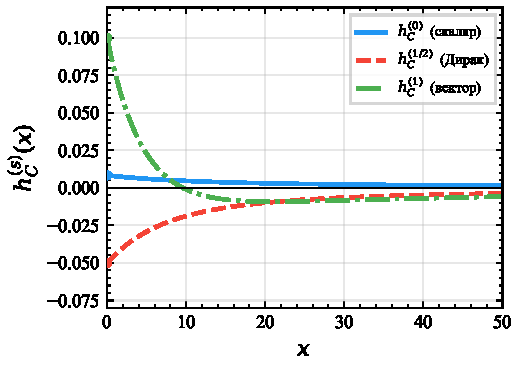
\includegraphics[width=0.8\textwidth]{figures/fig_hC_ru.pdf}
  \caption{Формфакторы квадрата тензора Вейля $h_C^{(s)}(x)$ для трёх спиновых
  секторов, где $x = \Box/\Lambda^2$. Локальные пределы:
  $h_C^{(0)}(0) = 1/120$ (скаляр, синий),
  $h_C^{(1/2)}(0) = -1/20$ (Дирак, красный) и
  $h_C^{(1)}(0) = 1/10$ (вектор, зелёный). Все формфакторы убывают как
  $1/x$ при $x \to \infty$.}
  \label{fig:hC}
\end{figure}

\begin{figure}[t]
  \centering
  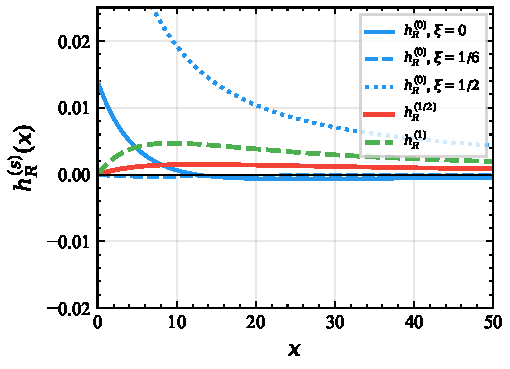
\includegraphics[width=0.8\textwidth]{figures/fig_hR_ru.pdf}
  \caption{Формфакторы $R^2$: $h_R^{(s)}(x)$, где $x = \Box/\Lambda^2$.
  Скалярный формфактор (синий) зависит от
  параметра неминимальной связи $\xi$: он тождественно обращается в нуль при
  конформной связи $\xi = 1/6$ (штриховая линия) и растёт с~увеличением
  $|\xi - 1/6|$. Вклады дираковского фермиона (красный) и вектора (зелёный)
  не зависят от $\xi$ и начинаются с~$h_R(0) = 0$.}
  \label{fig:hR}
\end{figure}


% ============================================================
\section{Сборка Стандартной модели}
\label{sec:sm}
% ============================================================

\subsection{Содержание частиц}

Содержание полей СМ, входящее в однопетлевое спектральное действие:
\begin{center}
\renewcommand{\arraystretch}{1.2}
\begin{tabular}{@{}lcc@{}}
  \toprule
  Тип частиц & Число & Обозначение \\
  \midrule
  Вещественные скаляры (дублет Хиггса) & 4 & $N_s = 4$ \\
  Вейлевские фермионы (3 поколения) & 45 & $N_f = 45$ \\
  Калибровочные бозоны ($8+3+1$) & 12 & $N_v = 12$ \\
  \bottomrule
\end{tabular}
\end{center}

Поскольку формфакторы из разд.~\ref{sec:dirac} определены на один
4-компонентный дираковский фермион, эффективное число дираковских фермионов
равно $N_D = N_f/2 = 45/2$ в~соответствии с~соглашением~\cite{Codello:2008vh}.

\subsection{Полный коэффициент при тензоре Вейля}

Полный формфактор квадрата тензора Вейля:
\begin{equation}
  \alpha_C(z) = N_s\,h_C^{(0)}(z) + N_D\,h_C^{(1/2)}(z)
    + N_v\,h_C^{(1)}(z)\,.
  \label{eq:alphaC-z}
\end{equation}
При $z = 0$:
\begin{align}
  \alpha_C &= 4 \cdot \frac{1}{120}
    + \frac{45}{2}\cdot\!\left(-\frac{1}{20}\right)
    + 12 \cdot \frac{1}{10} \nonumber\\
  &= \frac{4 - 135 + 144}{120}\,,
  \label{eq:alphaC-sum}
\end{align}
что даёт центральный результат:
\begin{equation}
  \boxed{\alpha_C = \frac{13}{120} \approx 0{,}1083\,.}
  \label{eq:alphaC}
\end{equation}

Эта величина положительна и не зависит от~$\xi$. Знаковая структура
($+4 - 135 + 144$) показывает, что вклад векторного сектора ($+144/120$)
преобладает над вкладом фермионного сектора ($-135/120$) с~запасом $+9/120$,
в~то время как скалярный сектор вносит $+4/120$. Положительность $\alpha_C$
означает, что спин-2 гравитационная мода в линеаризованной теории является
духом~\cite{Stelle:1976gc} --- хорошо известная особенность квадратичной
гравитации.

\subsection{Полный коэффициент при \texorpdfstring{$R^2$}{R2}}

\begin{align}
  \alpha_R(\xi) &= N_s \cdot \frac{1}{2}\!\left(\xi - \frac{1}{6}\right)^{\!2}
    + N_D \cdot 0 + N_v \cdot 0\,,
\end{align}
откуда
\begin{equation}
  \boxed{\alpha_R(\xi) = 2\!\left(\xi - \frac{1}{6}\right)^{\!2}\,.}
  \label{eq:alphaR}
\end{equation}

Вклад вносит только скалярный сектор: $\beta_R$ для фермиона Дирака и
для максвелловского поля обращаются в нуль в~силу конформной инвариантности.
Результат представляет собой полный квадрат, поэтому
$\alpha_R(\xi) \geq 0$ для всех~$\xi$, причём $\alpha_R(1/6) = 0$ при
конформной связи.

\subsection{Пересчёт базиса и \texorpdfstring{$c_1/c_2$}{c1/c2}}

Используя тождество Гаусса--Бонне для перехода к базису
$\{R^2, R_{\mu\nu}^2\}$ ($C^2 = 2R_{\mu\nu}^2 - \frac{2}{3}R^2$ с точностью
до топологической плотности Эйлера), получаем $c_1 = \alpha_R - \frac{2}{3}\alpha_C$
и $c_2 = 2\alpha_C$, что даёт
\begin{equation}
  \boxed{\frac{c_1}{c_2} = -\frac{1}{3}
    + \frac{120\!\left(\xi - \frac{1}{6}\right)^{\!2}}{13}\,.}
  \label{eq:c1c2}
\end{equation}

При конформной связи $\xi = 1/6$ это сводится к $c_1/c_2 = -1/3$. При
минимальной связи $\xi = 0$ получаем $c_1/c_2 = -1/13$.

\subsection{Отщепление скалярной моды}

Комбинация $3c_1 + c_2$ определяет массу скалярного гравитона
($m_0^2 \propto \Lambda^2/(3c_1 + c_2)$). Прямое вычисление даёт
\begin{equation}
  3c_1 + c_2 = 3\alpha_R(\xi) = 6\!\left(\xi - \frac{1}{6}\right)^{\!2}\,.
  \label{eq:3c1c2}
\end{equation}
Скалярная мода отщепляется (бесконечная масса) тогда и только тогда, когда
$\xi = 1/6$, что обеспечивает динамический механизм исключения скалярного
сектора гравитона через конформную связь поля Хиггса.

\begin{table}[t]
\caption{Сводка основных результатов. Все величины определены в тексте;
$\Lambda$ --- спектральный масштаб обрезания, а $\xi$ --- параметр
неминимальной связи Хиггса.}
\label{tab:summary}
\centering
\renewcommand{\arraystretch}{1.2}
\begin{tabular}{@{}lll@{}}
\toprule
Величина & Значение & Ур. \\
\midrule
$\alpha_C$ & $13/120 \approx 0{,}1083$ & (\ref{eq:alphaC}) \\
$\alpha_R(\xi)$ & $2(\xi - 1/6)^2$ & (\ref{eq:alphaR}) \\
$c_1/c_2$ & $-1/3 + 120(\xi - 1/6)^2/13$ & (\ref{eq:c1c2}) \\
$3c_1 + c_2$ & $6(\xi - 1/6)^2$ & (\ref{eq:3c1c2}) \\
$\lim_{x\to\infty} x\,\alpha_C$ & $-89/12$ & (\ref{eq:uv-coeff}) \\
$m_2$ & $\Lambda\sqrt{60/13} \approx 2{,}148\,\Lambda$ & (\ref{eq:m2}) \\
$m_0\,(\xi=0)$ & $\Lambda\sqrt{6} \approx 2{,}449\,\Lambda$ & (\ref{eq:m0}) \\
$m_2/m_0\,|_{\xi=0}$ & $\sqrt{10/13} \approx 0{,}877$ & (\ref{eq:mass-ratio}) \\
$V(0)/V_{\text{N}}(0)$ & $0$ (конечен в начале координат) & (\ref{eq:V-ratio}) \\
\bottomrule
\end{tabular}
\end{table}

\begin{figure}[t]
  \centering
  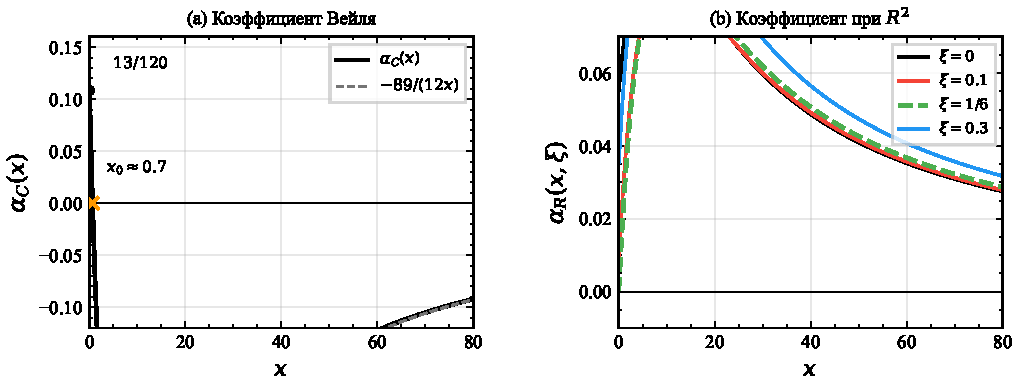
\includegraphics[width=\textwidth]{figures/fig_alpha_total_ru.pdf}
  \caption{Полные суммы Стандартной модели как функции $x = \Box/\Lambda^2$.
  (a)~Коэффициент при тензоре Вейля $\alpha_C(x)$ начинается с~$13/120$ и
  пересекает нуль при $x_0 \approx 0{,}7$, стремясь к~асимптоте $-89/(12x)$
  (штриховая серая линия) при $x \gg 1$. Смена знака сигнализирует о~переходе
  в~эффективной связи при квадрате тензора Вейля.
  (b)~Коэффициент при $R^2$: $\alpha_R(x,\xi)$ для нескольких значений
  параметра неминимальной связи Хиггса~$\xi$. При конформной связи $\xi = 1/6$
  (зелёная штриховая линия) $\alpha_R$ обращается в нуль при $x = 0$ и остаётся
  малым при всех~$x$.}
  \label{fig:alpha}
\end{figure}


% ============================================================
\section{Свойства формфакторов}
\label{sec:properties}
% ============================================================

\subsection{Природа целых функций}

Поскольку $\varphi(z)$ является целой функцией первого порядка [её ряд Тейлора
имеет бесконечный радиус сходимости, ср.~ур.~\eqref{eq:phi-def}], а
формфакторы \eqref{eq:hC0}--\eqref{eq:hR1} представляют собой рациональные
комбинации $\varphi$ и $1/z$, все кажущиеся особенности при $z = 0$ устранимы
(проверено по правилу Лопиталя), и каждый $h_C^{(s)}(z)$ и $h_R^{(s)}(z)$
является целой функцией. По линейности полные суммы СМ $\alpha_C(z)$ и
$\alpha_R(z,\xi)$ также являются целыми функциями переменной~$z$.

Физически формфакторы спектрального действия, таким образом, не вносят
\emph{новых полюсов} в пропагатор гравитона помимо классических. Любые
полюса духов возникают исключительно из нулей одетого пропагатора
$\Pi_{TT}(z) = 1 + \frac{13}{60}\,z\,\hat{F}_1(z)$, а не из особенностей
самих $F_1$ или~$F_2$.

\subsection{Ультрафиолетовая асимптотика}

При $x \to \infty$ имеем $\varphi(x) \to 2/x + O(1/x^2)$, откуда
\begin{align}
  x\,h_C^{(0)} &\to \frac{1}{12}\,,\quad
  x\,h_C^{(1/2)} \to -\frac{1}{6}\,,\quad
  x\,h_C^{(1)} \to -\frac{1}{3}\,.
\end{align}
Полный ультрафиолетовый коэффициент:
\begin{equation}
  \lim_{x\to\infty} x\,\alpha_C(x)
    = \frac{4}{12} - \frac{45}{12} - \frac{48}{12}
    = -\frac{89}{12}\,.
  \label{eq:uv-coeff}
\end{equation}

Смена знака от $\alpha_C(0) = +13/120$ к
$x\,\alpha_C \to -89/12 < 0$ означает, что $\alpha_C(z)$ пересекает нуль
при конечном $z_0 \approx 0{,}7$ (рис.~\ref{fig:alpha}a), сигнализируя
о~переходе в~эффективном знаке связи при квадрате тензора Вейля.

\subsection{Эффективные массы гравитонов}
\label{sec:masses}

В~линеаризованной теории на плоском фоне одетые пропагаторы спина 2 и спина 0
имеют вид
\begin{align}
  G_{TT} &\propto \frac{1}{k^2\,\Pi_{TT}(k^2/\Lambda^2)}\,,\\
  G_s &\propto \frac{1}{k^2\,\Pi_s(k^2/\Lambda^2,\xi)}\,,
\end{align}
где $\Pi_{TT}(z) = 1 + (13/60)\,z\,\hat{F}_1(z)$ и
$\Pi_s(z,\xi) = 1 + 6(\xi - 1/6)^2\,z\,\hat{F}_2(z,\xi)$. Разложение вблизи
$z = 0$ при $\hat{F}_1(0) = 1$ даёт:
\begin{equation}
  m_2 = \Lambda\sqrt{\frac{60}{13}} \approx 2{,}148\,\Lambda\,,
  \label{eq:m2}
\end{equation}
а при $\xi \neq 1/6$:
\begin{equation}
  m_0(\xi) = \frac{\Lambda}{\sqrt{6(\xi - 1/6)^2}}\,.
  \label{eq:m0}
\end{equation}
При минимальной связи $\xi = 0$ это даёт
$m_0 = \Lambda\sqrt{6} \approx 2{,}449\,\Lambda$. Отношение масс
\begin{equation}
  \frac{m_2}{m_0}\bigg|_{\xi=0} = \sqrt{\frac{10}{13}} \approx 0{,}877
  \label{eq:mass-ratio}
\end{equation}
фиксировано содержанием частиц СМ и не зависит от~$\Lambda$.

Модифицированный ньютоновский потенциал в линеаризованной
теории~\cite{Stelle:1976gc}:
\begin{equation}
  \frac{V(r)}{V_{\text{N}}(r)}
  = 1 - \frac{4}{3}\,e^{-m_2 r} + \frac{1}{3}\,e^{-m_0 r}\,,
  \label{eq:V-ratio}
\end{equation}
который показан на рис.~\ref{fig:potential}. При $r = 0$ экспоненты
компенсируются, давая $V(0) = 0$ и конечный гравитационный потенциал в начале
координат. Закон Ньютона восстанавливается при $r \gg 1/\Lambda$.

\begin{figure}[t]
  \centering
  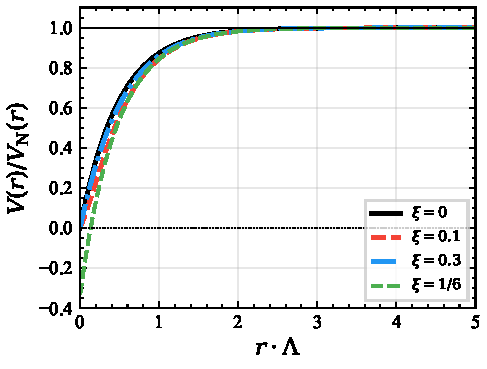
\includegraphics[width=0.8\textwidth]{figures/fig_potential_ru.pdf}
  \caption{Модифицированный ньютоновский потенциал $V(r)/V_{\text{N}}(r)$ для
  нескольких значений~$\xi$ как функция $r\Lambda$. При конформной
  связи $\xi = 1/6$ (зелёная штриховая линия) скалярная мода отщепляется, и
  потенциал опускается до $-1/3$ прежде, чем восстановится закон Ньютона.
  Для всех~$\xi$ $V(0) = 0$ (конечен в начале координат) и $V \to V_{\text{N}}$
  при $r \gg 1/\Lambda$.}
  \label{fig:potential}
\end{figure}


% ============================================================
\section{Обсуждение}
\label{sec:discussion}
% ============================================================

\subsection{Сравнение с~существующими результатами}

Локальные пределы ($\beta_W^{(s)}, \beta_R^{(s)}$) согласуются
с~установленными результатами
работ~\cite{Stelle:1976gc,Codello:2008vh,Parker:2009uva,Avramidi:2000bm},
сведёнными в таблицу~\ref{tab:beta}.
В~частности, коэффициент при тензоре Вейля для СМ, $13/120$, может быть
разложен как
\begin{equation}
  \frac{13}{120} = \frac{N_s}{120}
    - \frac{N_D}{20} + \frac{N_v}{10}\,,
\end{equation}
что совпадает с~общей формулой из~\cite{Codello:2008vh} при
$\delta_s = 1/120$, $|\delta_f| = 1/20$ (на один дираковский фермион,
без знака в их соглашении) и $\delta_v = 1/10$ (на один калибровочный бозон,
после вычитания духов).

Нелокальные формфакторы $h_C^{(s)}(x)$ и $h_R^{(s)}(x)$ сводятся к~выражениям
КЗ~\cite{Codello:2012kq} при указании эндоморфизма Лихнеровича
$E = -R/4$ для дираковского сектора и числа вычитаемых духов, равного~2, для
сектора калибровочных бозонов.

\begin{table}[t]
\caption{Однопетлевые коэффициенты $\beta$-функции $\beta_W^{(s)} \equiv
h_C^{(s)}(0)$ и $\beta_R^{(s)} \equiv h_R^{(s)}(0)$ для каждого спинового
сектора в сравнении с литературой. Знаковое соглашение для спина 1/2 явно
включает множитель $(-1)^{2s}$; КПР~\cite{Codello:2008vh} приводят значение
без знака $|\beta_W^{(1/2)}| = 1/20$.
КЗ~=~Коделло--Занусси~\cite{Codello:2012kq},
ПТ~=~Паркер--Томс~\cite{Parker:2009uva},
С77~=~Стелле~\cite{Stelle:1976gc}.}
\label{tab:beta}
\centering
\renewcommand{\arraystretch}{1.3}
\begin{tabular}{@{}lcccc@{}}
\toprule
Спин & $\beta_W^{(s)}$ & Лит. & $\beta_R^{(s)}$ & Лит. \\
\midrule
$0$ & $\frac{1}{120}$ & КЗ, ПТ &
  $\frac{1}{2}\!\left(\xi\!-\!\frac{1}{6}\right)^{\!2}$ & ПТ \\[3pt]
$\frac{1}{2}$ & $-\frac{1}{20}$ & КЗ, КПР &
  $0$ & КЗ, ПТ \\[3pt]
$1$ & $\frac{1}{10}$ & С77, КПР &
  $0$ & КЗ, ПТ \\[3pt]
\midrule
СМ & $\frac{13}{120}$ & -- &
  $2\!\left(\xi\!-\!\frac{1}{6}\right)^{\!2}$ & -- \\
\bottomrule
\end{tabular}
\end{table}

\subsection{Роль неминимальной связи}

Параметр~$\xi$ входит исключительно через скалярный сектор и влияет
только на~$\alpha_R$ (но не на~$\alpha_C$). Это имеет два следствия:
\begin{enumerate}
\item Спектр спин-2 гравитона ($\Pi_{TT}$, массы духов, ультрафиолетовое
  поведение) полностью не зависит от~$\xi$ и, следовательно, является
  устойчивым следствием формализма.
\item Скалярный сектор гравитона управляем: при $\xi = 1/6$ весь сектор~$R^2$
  обращается в нуль, и скалярная мода отщепляется. Это обеспечивает
  естественное разрешение проблемы скалярного духа через конформную связь.
\end{enumerate}

\subsection{Лоренцево продолжение}

Вычисленные здесь формфакторы являются евклидовыми ($\Box_E > 0$). Лоренцевы
формфакторы получаются вик-поворотом $z_E \to -z_L$, т.\,е.\
$F_i(\Box_E/\Lambda^2) \to F_i(-\Box_L/\Lambda^2)$. Поскольку $\varphi(z)$
является целой функцией, это продолжение корректно определено для всех~$z$.
Полюса одетого пропагатора (массы духов) находятся из решения уравнения
$\Pi_{TT}(-z_L) = 0$ и обсуждаются в~сопровождающей статье.

\subsection{Следствия для нелокальной гравитации}

Природа целых функций формфакторов связывает спектральное действие
с~программой нелокальной гравитации (гравитации с бесконечным числом
производных)~\cite{Modesto:2011kw,Tomboulis:1997gg,Biswas:2011ar}, где целые
функции от~$\Box$ вводятся для улучшения ультрафиолетового поведения.
В~спектральном действии эти формфакторы возникают \emph{производным} образом
из ядра теплопроводности, а не постулируются. Однопетлевая степень расходимости
снижается с~$D = 4$ (гравитация Эйнштейна) до $D = 0$ (логарифмическая), что
согласуется с~результатами~\cite{Stelle:1976gc} для локальной квадратичной
гравитации, но с~дополнительной структурой зависящих от импульса формфакторов,
модифицирующих ультрафиолетовое поведение на всех масштабах.


% ============================================================
\section{Заключение}
\label{sec:conclusions}
% ============================================================

Мы вычислили полные нелокальные однопетлевые формфакторы спектрального действия
со~всем содержанием частиц Стандартной модели. Центральными результатами
являются определяемый СМ коэффициент при тензоре Вейля $\alpha_C = 13/120$ и
зависящий от~$\xi$ коэффициент при $R^2$:
$\alpha_R(\xi) = 2(\xi - 1/6)^2$, а~также замкнутые
выражения~\eqref{eq:scalar-ff}--\eqref{eq:vector-ff}
для каждого спинового сектора.

Формфакторы являются целыми функциями переменной $\Box/\Lambda^2$, что
гарантирует отсутствие новых полюсов пропагатора, и дают эффективные массы
гравитонов $m_2 = \Lambda\sqrt{60/13}$ (спин~2) и
$m_0 = \Lambda/\sqrt{6(\xi-1/6)^2}$ (спин~0), определяемые спектром СМ.
Скалярный гравитон отщепляется при конформной связи $\xi = 1/6$, а
ультрафиолетовое поведение является логарифмическим ($D = 0$), что улучшает
ситуацию по сравнению с~гравитацией Эйнштейна ($D = 4$).

Полученные результаты закладывают основу для систематического исследования
квантово-гравитационной феноменологии спектрального действия, включая
модифицированный ньютоновский потенциал, параметризованное
постньютоновское приближение (ПП-параметры), распространение гравитационных волн
и структуру унитарности, которые будут представлены в~сопровождающих статьях.


% ============================================================
\section*{Благодарности}
% ============================================================
Все символьные результаты были проверены численно с~точностью
$\geq 100$ значащих цифр с~помощью \texttt{mpmath}~и сопоставлены
с~оригинальными выражениями КЗ из~\cite{Codello:2012kq} и коэффициентами
Сили--ДеВитта из~\cite{Vassilevich:2003xt,Avramidi:2000bm}.

\section*{Доступность данных}
Вычислительные инструменты, использованные в~данной работе, включая реализации
всех формфакторов с~произвольной точностью, доступны у~автора по обоснованному
запросу.


\begin{thebibliography}{18}

\bibitem{Chamseddine:1996zu} Chamseddine~A.\,H., Connes~A. The spectral action principle. \textit{Commun. Math. Phys.} \textbf{186}, 731--750 (1997). \url{https://doi.org/10.1007/s002200050126}

\bibitem{Chamseddine:2006ep} Chamseddine~A.\,H., Connes~A. Inner fluctuations of the spectral action. \textit{J. Geom. Phys.} \textbf{57}, 1--21 (2006). \url{https://doi.org/10.1016/j.geomphys.2006.08.003}

\bibitem{Chamseddine:2010ud} Chamseddine~A.\,H., Connes~A. Noncommutative geometry as a framework for unification of all fundamental interactions including gravity. Part~I. \textit{Fortsch. Phys.} \textbf{58}, 553--600 (2010). \url{https://doi.org/10.1002/prop.201000069}

\bibitem{vanSuijlekom:2014pya} van Suijlekom~W.\,D. \textit{Noncommutative Geometry and Particle Physics}. Dordrecht, Springer (2015). \url{https://doi.org/10.1007/978-94-017-9162-5}

\bibitem{Barvinsky:1985an} Barvinsky~A.\,O., Vilkovisky~G.\,A. The generalized Schwinger-DeWitt technique in gauge theories and quantum gravity. \textit{Phys. Rept.} \textbf{119}, 1--74 (1985). \url{https://doi.org/10.1016/0370-1573(85)90148-6}

\bibitem{Barvinsky:1987uw} Barvinsky~A.\,O., Vilkovisky~G.\,A. Beyond the Schwinger-DeWitt technique: converting loops into trees and in-in currents. \textit{Nucl. Phys. B} \textbf{282}, 163--188 (1987). \url{https://doi.org/10.1016/0550-3213(87)90681-X}

\bibitem{Codello:2012kq} Codello~A., Zanusso~O. On the non-local heat kernel expansion. \textit{J. Math. Phys.} \textbf{54}, 013513 (2013). \url{https://doi.org/10.1063/1.4776234}

\bibitem{DeWitt:1964mxt} DeWitt~B.\,S. Dynamical theory of groups and fields. In: \textit{Conf. Proc. C} \textbf{630701}, 585--820 (1964).

\bibitem{Gilkey:1975iq} Gilkey~P.\,B. The spectral geometry of a Riemannian manifold. \textit{J. Diff. Geom.} \textbf{10}~(4), 601--618 (1975).

\bibitem{Vassilevich:2003xt} Vassilevich~D.\,V. Heat kernel expansion: user's manual. \textit{Phys. Rept.} \textbf{388}, 279--360 (2003). \url{https://doi.org/10.1016/j.physrep.2003.09.002}

\bibitem{Avramidi:2000bm} Avramidi~I.\,G. Heat kernel approach in quantum field theory. \textit{Nucl. Phys. B Proc. Suppl.} \textbf{104}, 3--32 (2002). \url{https://doi.org/10.1016/S0920-5632(01)01593-6}

\bibitem{Fursaev:2011zz} Fursaev~D.\,V., Vassilevich~D.\,V. \textit{Operators, Geometry and Quanta: Methods of Spectral Geometry in Quantum Field Theory}. Dordrecht, Springer (2011). \url{https://doi.org/10.1007/978-94-007-0205-9}

\bibitem{Codello:2008vh} Codello~A., Percacci~R., Rahmede~C. Investigating the ultraviolet properties of gravity with a Wilsonian renormalization group equation. \textit{Annals Phys.} \textbf{324}, 414--469 (2009). \url{https://doi.org/10.1016/j.aop.2008.08.008}

\bibitem{Parker:2009uva} Parker~L., Toms~D. \textit{Quantum Field Theory in Curved Spacetime: Quantized Fields and Gravity}. Cambridge, Cambridge University Press (2009). \url{https://doi.org/10.1017/CBO9780511813924}

\bibitem{Stelle:1976gc} Stelle~K.\,S. Renormalization of higher-derivative quantum gravity. \textit{Phys. Rev. D} \textbf{16}, 953--969 (1977). \url{https://doi.org/10.1103/PhysRevD.16.953}

\bibitem{Modesto:2011kw} Modesto~L. Super-renormalizable quantum gravity. \textit{Phys. Rev. D} \textbf{86}, 044005 (2012). \url{https://doi.org/10.1103/PhysRevD.86.044005}

\bibitem{Tomboulis:1997gg} Tomboulis~E.\,T. Superrenormalizable gauge and gravitational theories. arXiv:hep-th/9702146 (1997).

\bibitem{Biswas:2011ar} Biswas~T., Gerber~E., Mazumdar~A., Talaganis~S. Towards singularity- and ghost-free theories of gravity. \textit{Phys. Rev. Lett.} \textbf{108}, 031101 (2012). \url{https://doi.org/10.1103/PhysRevLett.108.031101}

\end{thebibliography}

\end{document}
